% !TeX program = xelatex
% A single continuous flowchart drawn from nodes and arrows, with no imported pages or images.
% Compile this standalone source using XeLaTeX.
\RequirePackage{fix-cm}
\documentclass[10pt]{article}
\usepackage[paperwidth=348mm,paperheight=1080mm,margin=10mm]{geometry}
\usepackage{fontspec}
\setsansfont{texgyreheros}[Extension=.otf,UprightFont=*-regular,BoldFont=*-bold]
\setmonofont{lmmono10-regular.otf}[BoldFont=lmmonolt10-bold.otf]
\renewcommand{\familydefault}{\sfdefault}
\usepackage{tikz}
\usetikzlibrary{arrows.meta}
\definecolor{Navy}{HTML}{17324D}
\definecolor{Teal}{HTML}{007F82}
\definecolor{Amber}{HTML}{936219}
\pagestyle{empty}
\setlength{\parindent}{0pt}
\tikzset{
 agent/.style={rounded corners=2mm,draw=Teal!70,fill=Teal!5,line width=.8pt,align=left,text=Navy,inner sep=3.5mm},
 coord/.style={agent,draw=Navy!55,fill=Navy!4},
 note/.style={agent,draw=Amber!50,fill=Amber!5},
 human/.style={agent,draw=Teal,line width=1.2pt,fill=Teal!13,align=center},
 decision/.style={draw=Amber,fill=Amber!7,line width=.9pt},
 flow/.style={-{Stealth[length=2.6mm,width=1.7mm]},draw=Navy!80,line width=1pt,rounded corners=1mm},
 tag/.style={fill=white,text=Navy,font=\fontsize{9.3}{11.5}\selectfont,align=center,inner sep=1mm}
}
\begin{document}
\noindent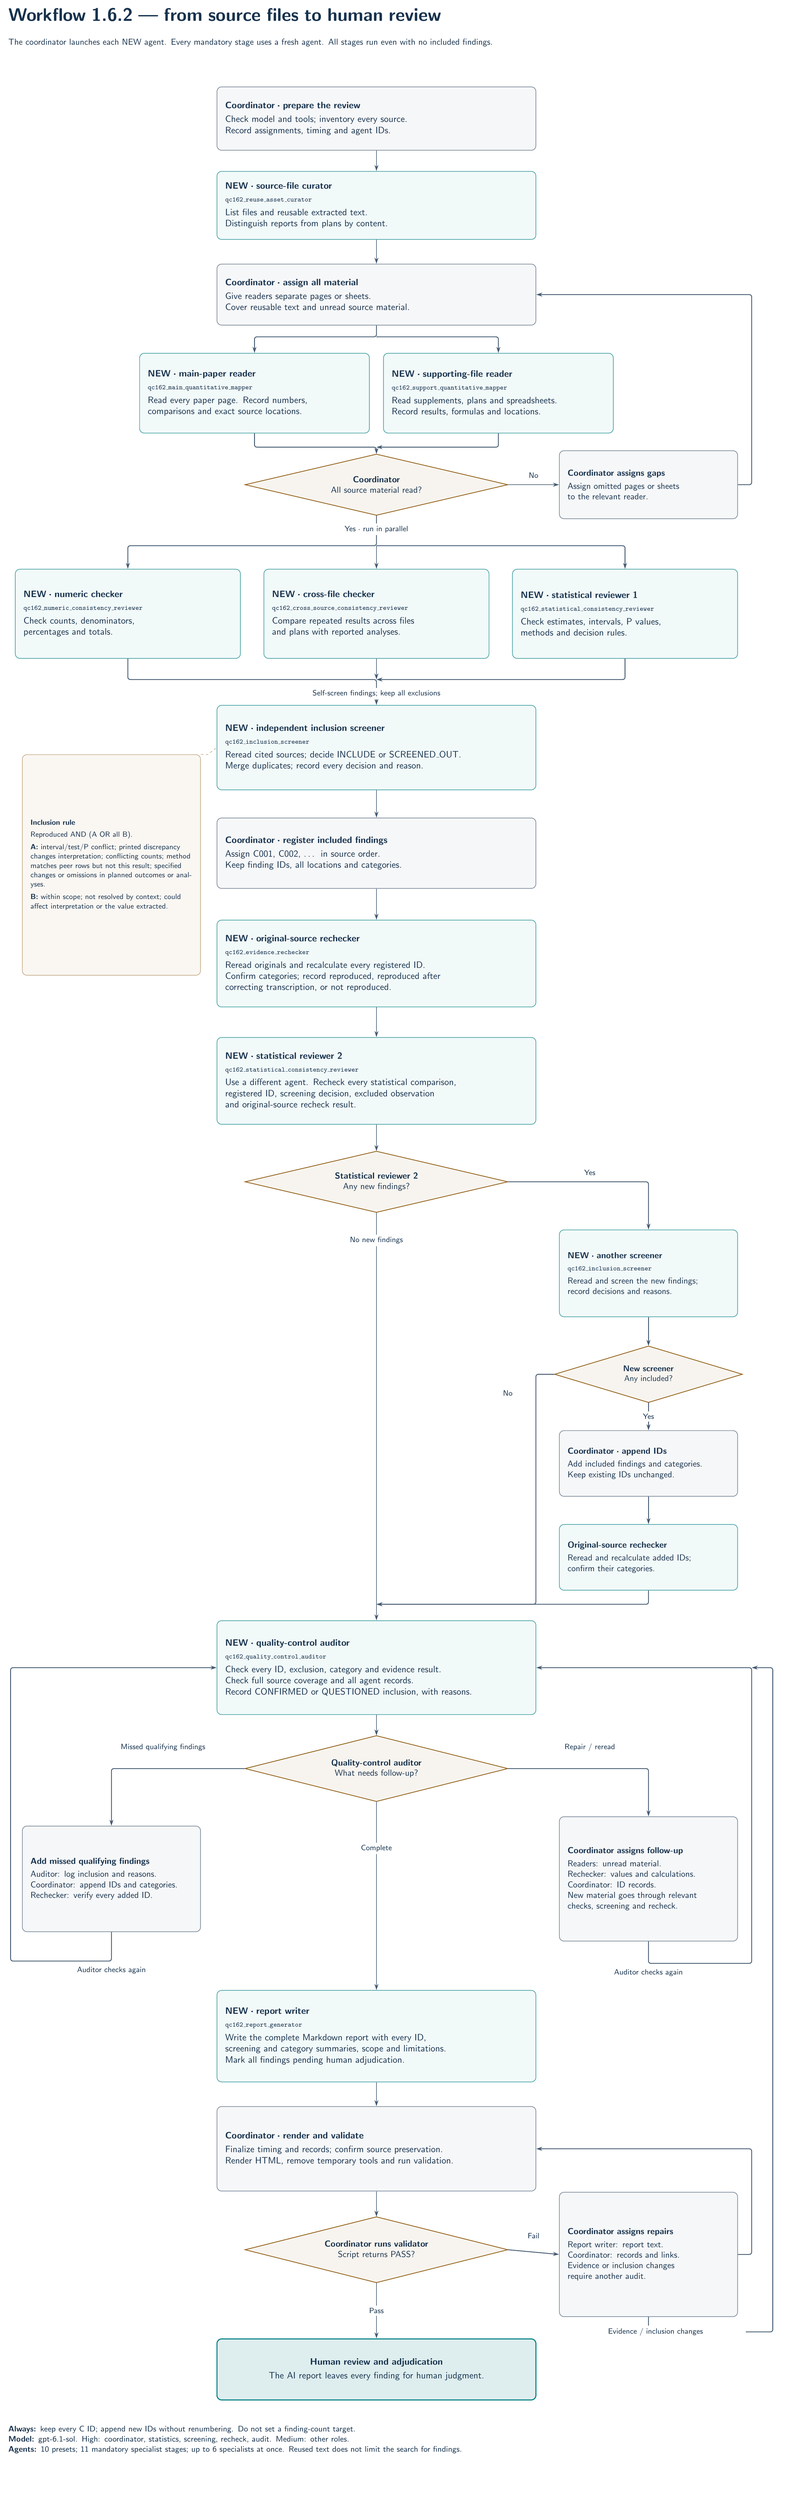
\begin{tikzpicture}[x=1mm,y=-1mm]
\path[use as bounding box] (0,0) rectangle (328,1058);
\node[anchor=north west,align=left,text=Navy,inner sep=0,text width=328mm,font=\fontsize{22}{24.5}\selectfont] at (0,0) {{\fontsize{22}{26}\selectfont\bfseries Workflow 1.6.2 — from source files to human review}};
\node[anchor=north west,align=left,text=Navy,inner sep=0,text width=328mm,font=\fontsize{10.5}{13.0}\selectfont] at (0,13) {The coordinator launches each NEW agent. Every mandatory stage uses a fresh agent. All stages run even with no included findings.};
\node[coord,text width=129mm,minimum width=136mm,minimum height=27mm,font=\fontsize{11.2}{13.5}\selectfont] (setup) at (157,47) {\textbf{Coordinator · prepare the review}\\[3pt]Check model and tools; inventory every source.\\Record assignments, timing and agent IDs.};
\node[agent,text width=129mm,minimum width=136mm,minimum height=29mm,font=\fontsize{11.2}{13.5}\selectfont] (curator) at (157,84) {\textbf{NEW · source-file curator}\\[2pt]{\normalfont\ttfamily\fontsize{8.2}{10}\selectfont qc162\_reuse\_asset\_curator}\\[3pt]List files and reusable extracted text.\\Distinguish reports from plans by content.};
\node[coord,text width=129mm,minimum width=136mm,minimum height=26mm,font=\fontsize{11.2}{13.5}\selectfont] (assign) at (157,122) {\textbf{Coordinator · assign all material}\\[3pt]Give readers separate pages or sheets.\\Cover reusable text and unread source material.};
\node[agent,text width=91mm,minimum width=98mm,minimum height=34mm,font=\fontsize{11.2}{13.5}\selectfont] (main) at (105,164) {\textbf{NEW · main-paper reader}\\[2pt]{\normalfont\ttfamily\fontsize{8.2}{10}\selectfont qc162\_main\_quantitative\_mapper}\\[3pt]Read every paper page. Record numbers,\\comparisons and exact source locations.};
\node[agent,text width=91mm,minimum width=98mm,minimum height=34mm,font=\fontsize{11.2}{13.5}\selectfont] (support) at (209,164) {\textbf{NEW · supporting-file reader}\\[2pt]{\normalfont\ttfamily\fontsize{8.2}{10}\selectfont qc162\_support\_quantitative\_mapper}\\[3pt]Read supplements, plans and spreadsheets.\\Record results, formulas and locations.};
\draw[decision] (101.0,203) -- (157,190.0) -- (213.0,203) -- (157,216.0) -- cycle;
\node[align=center,text=Navy,inner sep=0,text width=92mm,minimum width=112mm,minimum height=26mm,font=\fontsize{10.6}{12.6}\selectfont] (coverage) at (157,203) {\textbf{Coordinator}\\All source material read?};
\node[coord,text width=69mm,minimum width=76mm,minimum height=29mm,font=\fontsize{10.5}{12.8}\selectfont] (gap) at (273,203) {\textbf{Coordinator assigns gaps}\\[3pt]Assign omitted pages or sheets\\to the relevant reader.};
\node[agent,text width=89mm,minimum width=96mm,minimum height=38mm,font=\fontsize{11.2}{13.5}\selectfont] (num) at (51,258) {\textbf{NEW · numeric checker}\\[2pt]{\normalfont\ttfamily\fontsize{8.2}{10}\selectfont qc162\_numeric\_consistency\_reviewer}\\[3pt]Check counts, denominators,\\percentages and totals.};
\node[agent,text width=89mm,minimum width=96mm,minimum height=38mm,font=\fontsize{11.2}{13.5}\selectfont] (cross) at (157,258) {\textbf{NEW · cross-file checker}\\[2pt]{\normalfont\ttfamily\fontsize{8.2}{10}\selectfont qc162\_cross\_source\_consistency\_reviewer}\\[3pt]Compare repeated results across files\\and plans with reported analyses.};
\node[agent,text width=89mm,minimum width=96mm,minimum height=38mm,font=\fontsize{11.2}{13.5}\selectfont] (statsone) at (263,258) {\textbf{NEW · statistical reviewer 1}\\[2pt]{\normalfont\ttfamily\fontsize{8.2}{10}\selectfont qc162\_statistical\_consistency\_reviewer}\\[3pt]Check estimates, intervals, P values,\\methods and decision rules.};
\node[agent,text width=129mm,minimum width=136mm,minimum height=36mm,font=\fontsize{11.2}{13.5}\selectfont] (screen) at (157,315) {\textbf{NEW · independent inclusion screener}\\[2pt]{\normalfont\ttfamily\fontsize{8.2}{10}\selectfont qc162\_inclusion\_screener}\\[3pt]Reread cited sources; decide INCLUDE or SCREENED\_OUT.\\Merge duplicates; record every decision and reason.};
\node[coord,text width=129mm,minimum width=136mm,minimum height=30mm,font=\fontsize{11.2}{13.5}\selectfont] (register) at (157,360) {\textbf{Coordinator · register included findings}\\[3pt]Assign C001, C002, … in source order.\\Keep finding IDs, all locations and categories.};
\node[agent,text width=129mm,minimum width=136mm,minimum height=37mm,font=\fontsize{11.2}{13.5}\selectfont] (recheck) at (157,407) {\textbf{NEW · original-source rechecker}\\[2pt]{\normalfont\ttfamily\fontsize{8.2}{10}\selectfont qc162\_evidence\_rechecker}\\[3pt]Reread originals and recalculate every registered ID.\\Confirm categories; record reproduced, reproduced after\\correcting transcription, or not reproduced.};
\node[agent,text width=129mm,minimum width=136mm,minimum height=37mm,font=\fontsize{11.2}{13.5}\selectfont] (statstwo) at (157,457) {\textbf{NEW · statistical reviewer 2}\\[2pt]{\normalfont\ttfamily\fontsize{8.2}{10}\selectfont qc162\_statistical\_consistency\_reviewer}\\[3pt]Use a different agent. Recheck every statistical comparison,\\registered ID, screening decision, excluded observation\\and original-source recheck result.};
\draw[decision] (101.0,500) -- (157,487.0) -- (213.0,500) -- (157,513.0) -- cycle;
\node[align=center,text=Navy,inner sep=0,text width=92mm,minimum width=112mm,minimum height=26mm,font=\fontsize{10.6}{12.6}\selectfont] (newfind) at (157,500) {\textbf{Statistical reviewer 2}\\Any new findings?};
\node[agent,text width=69mm,minimum width=76mm,minimum height=37mm,font=\fontsize{10.5}{12.8}\selectfont] (secondscreen) at (273,539) {\textbf{NEW · another screener}\\[2pt]{\normalfont\ttfamily\fontsize{8.2}{10}\selectfont qc162\_inclusion\_screener}\\[3pt]Reread and screen the new findings;\\record decisions and reasons.};
\draw[decision] (233.0,582) -- (273,570.0) -- (313.0,582) -- (273,594.0) -- cycle;
\node[align=center,text=Navy,inner sep=0,text width=60mm,minimum width=80mm,minimum height=24mm,font=\fontsize{10}{12}\selectfont] (included) at (273,582) {\textbf{New screener}\\Any included?};
\node[coord,text width=69mm,minimum width=76mm,minimum height=28mm,font=\fontsize{10.5}{12.8}\selectfont] (append) at (273,620) {\textbf{Coordinator · append IDs}\\[3pt]Add included findings and categories.\\Keep existing IDs unchanged.};
\node[agent,text width=69mm,minimum width=76mm,minimum height=28mm,font=\fontsize{10.5}{12.8}\selectfont] (extra) at (273,660) {\textbf{Original-source rechecker}\\[3pt]Reread and recalculate added IDs;\\confirm their categories.};
\node[agent,text width=129mm,minimum width=136mm,minimum height=40mm,font=\fontsize{11.2}{13.5}\selectfont] (audit) at (157,707) {\textbf{NEW · quality-control auditor}\\[2pt]{\normalfont\ttfamily\fontsize{8.2}{10}\selectfont qc162\_quality\_control\_auditor}\\[3pt]Check every ID, exclusion, category and evidence result.\\Check full source coverage and all agent records.\\Record CONFIRMED or QUESTIONED inclusion, with reasons.};
\draw[decision] (101.0,750) -- (157,736.0) -- (213.0,750) -- (157,764.0) -- cycle;
\node[align=center,text=Navy,inner sep=0,text width=92mm,minimum width=112mm,minimum height=28mm,font=\fontsize{10.6}{12.6}\selectfont] (followup) at (157,750) {\textbf{Quality-control auditor}\\What needs follow-up?};
\node[coord,text width=69mm,minimum width=76mm,minimum height=45mm,font=\fontsize{10.5}{12.8}\selectfont] (rescue) at (44,797) {\textbf{Add missed qualifying findings}\\[3pt]Auditor: log inclusion and reasons.\\Coordinator: append IDs and categories.\\Rechecker: verify every added ID.};
\node[coord,text width=69mm,minimum width=76mm,minimum height=53mm,font=\fontsize{10.5}{12.8}\selectfont] (auditfix) at (273,797) {\textbf{Coordinator assigns follow-up}\\[3pt]Readers: unread material.\\Rechecker: values and calculations.\\Coordinator: ID records.\\New material goes through relevant\\checks, screening and recheck.};
\node[agent,text width=129mm,minimum width=136mm,minimum height=39mm,font=\fontsize{11.2}{13.5}\selectfont] (report) at (157,864) {\textbf{NEW · report writer}\\[2pt]{\normalfont\ttfamily\fontsize{8.2}{10}\selectfont qc162\_report\_generator}\\[3pt]Write the complete Markdown report with every ID,\\screening and category summaries, scope and limitations.\\Mark all findings pending human adjudication.};
\node[coord,text width=129mm,minimum width=136mm,minimum height=36mm,font=\fontsize{11.2}{13.5}\selectfont] (render) at (157,912) {\textbf{Coordinator · render and validate}\\[3pt]Finalize timing and records; confirm source preservation.\\Render HTML, remove temporary tools and run validation.};
\draw[decision] (101.0,955) -- (157,941.0) -- (213.0,955) -- (157,969.0) -- cycle;
\node[align=center,text=Navy,inner sep=0,text width=92mm,minimum width=112mm,minimum height=28mm,font=\fontsize{10.6}{12.6}\selectfont] (valid) at (157,955) {\textbf{Coordinator runs validator}\\Script returns PASS?};
\node[coord,text width=69mm,minimum width=76mm,minimum height=53mm,font=\fontsize{10.5}{12.8}\selectfont] (filefix) at (273,957) {\textbf{Coordinator assigns repairs}\\[3pt]Report writer: report text.\\Coordinator: records and links.\\Evidence or inclusion changes\\require another audit.};
\node[human,text width=129mm,minimum width=136mm,minimum height=26mm,font=\fontsize{11.2}{13.5}\selectfont] (human) at (157,1006) {\textbf{Human review and adjudication}\\[3pt]The AI report leaves every finding for human judgment.};
\node[note,text width=69mm,minimum width=76mm,minimum height=94mm,font=\fontsize{9}{11.3}\selectfont] (rules) at (44,365) {\textbf{Inclusion rule}\\[3pt]Reproduced AND (A OR all B).\\[4pt]\textbf{A:} interval/test/P conflict; printed discrepancy changes interpretation; conflicting counts; method matches peer rows but not this result; specified changes or omissions in planned outcomes or analyses.\\[4pt]\textbf{B:} within scope; not resolved by context; could affect interpretation or the value extracted.};
\draw[draw=Amber!60,dashed,line width=.6pt] (rules.north east) -- (85,318) -- (screen.west);
\draw[flow] (setup.south) -- (curator.north);
\draw[flow] (curator.south) -- (assign.north);
\draw[flow] (assign.south) -- (157,140) -- (105,140) -- (main.north);
\draw[flow] (157,140) -- (209,140) -- (support.north);
\draw[flow] (main.south) -- (105,187) -- (157,187) -- (coverage.north);
\draw[flow] (support.south) -- (209,187) -- (157,187);
\draw[flow] (coverage.east) -- (gap.west);
\node[tag,text width=14mm] at (224,199) {No};
\draw[flow] (gap.east) -- (317,203) -- (317,122) -- (assign.east);
\draw[flow] (coverage.south) -- (157,229) -- (51,229) -- (num.north);
\draw[flow] (157,229) -- (cross.north);
\draw[flow] (157,229) -- (263,229) -- (statsone.north);
\node[tag,text width=52mm] at (157,222) {Yes · run in parallel};
\draw[flow] (num.south) -- (51,286) -- (157,286) -- (screen.north);
\draw[flow] (cross.south) -- (157,286);
\draw[flow] (statsone.south) -- (263,286) -- (157,286);
\node[tag,text width=100mm] at (157,292) {Self-screen findings; keep all exclusions};
\draw[flow] (screen.south) -- (register.north);
\draw[flow] (register.south) -- (recheck.north);
\draw[flow] (recheck.south) -- (statstwo.north);
\draw[flow] (statstwo.south) -- (newfind.north);
\draw[flow] (newfind.east) -- (273,500) -- (secondscreen.north);
\node[tag,text width=18mm] at (248,496) {Yes};
\draw[flow] (newfind.south) -- (audit.north);
\node[tag,text width=56mm] at (157,525) {No new findings};
\draw[flow] (secondscreen.south) -- (included.north);
\draw[flow] (included.south) -- (append.north);
\node[tag,text width=18mm] at (273,600) {Yes};
\draw[flow] (append.south) -- (extra.north);
\draw[flow] (included.west) -- (225,582) -- (225,680) -- (157,680);
\node[tag,text width=16mm] at (213,590) {No};
\draw[flow] (extra.south) -- (273,680) -- (157,680);
\draw[flow] (audit.south) -- (followup.north);
\draw[flow] (followup.west) -- (44,750) -- (rescue.north);
\node[tag,text width=55mm] at (66,741) {Missed qualifying findings};
\draw[flow] (followup.east) -- (273,750) -- (auditfix.north);
\node[tag,text width=49mm] at (248,741) {Repair / reread};
\draw[flow] (rescue.south) -- (44,832) -- (1,832) -- (1,707) -- (audit.west);
\draw[flow] (auditfix.south) -- (273,833) -- (317,833) -- (317,707) -- (audit.east);
\node[tag,text width=62mm] at (44,836) {Auditor checks again};
\node[tag,text width=64mm] at (273,837) {Auditor checks again};
\draw[flow] (followup.south) -- (report.north);
\node[tag,text width=56mm] at (157,784) {Complete};
\draw[flow] (report.south) -- (render.north);
\draw[flow] (render.south) -- (valid.north);
\draw[flow] (valid.east) -- (filefix.west);
\node[tag,text width=18mm] at (224,949) {Fail};
\draw[flow] (filefix.east) -- (317,957) -- (317,912) -- (render.east);
\draw[flow] (filefix.south) -- (273,990) -- (326,990) -- (326,707) -- (317,707);
\node[tag,text width=75mm] at (276,990) {Evidence / inclusion changes};
\draw[flow] (valid.south) -- (human.north);
\node[tag,text width=30mm] at (157,981) {Pass};
\node[anchor=north west,align=left,text=Navy,inner sep=0,text width=328mm,font=\fontsize{9.8}{12.3}\selectfont] at (0,1030) {\textbf{Always:} keep every C ID; append new IDs without renumbering. Do not set a finding-count target.\\\textbf{Model:} gpt-6.1-sol. High: coordinator, statistics, screening, recheck, audit. Medium: other roles.\\\textbf{Agents:} 10 presets; 11 mandatory specialist stages; up to 6 specialists at once. Reused text does not limit the search for findings.};
\end{tikzpicture}\end{document}
